\chapter{Entwicklung des Prototpys für Visual Studio Code}
\label{cha:EntwicklungVsCode}

\section{Design}
\label{sec:EntwicklungVsCode_Design}

Um das in Kapitel \ref{cha:Prototyp} beschriebene Plugin in VS Code
zu entwickeln, werden die Komponenten verwendet, die auch in 
Abbildung \ref{fig:diagram_VSCodeDesign-Simplified} abgebildet sind.
\begin{figure}
    \centering
    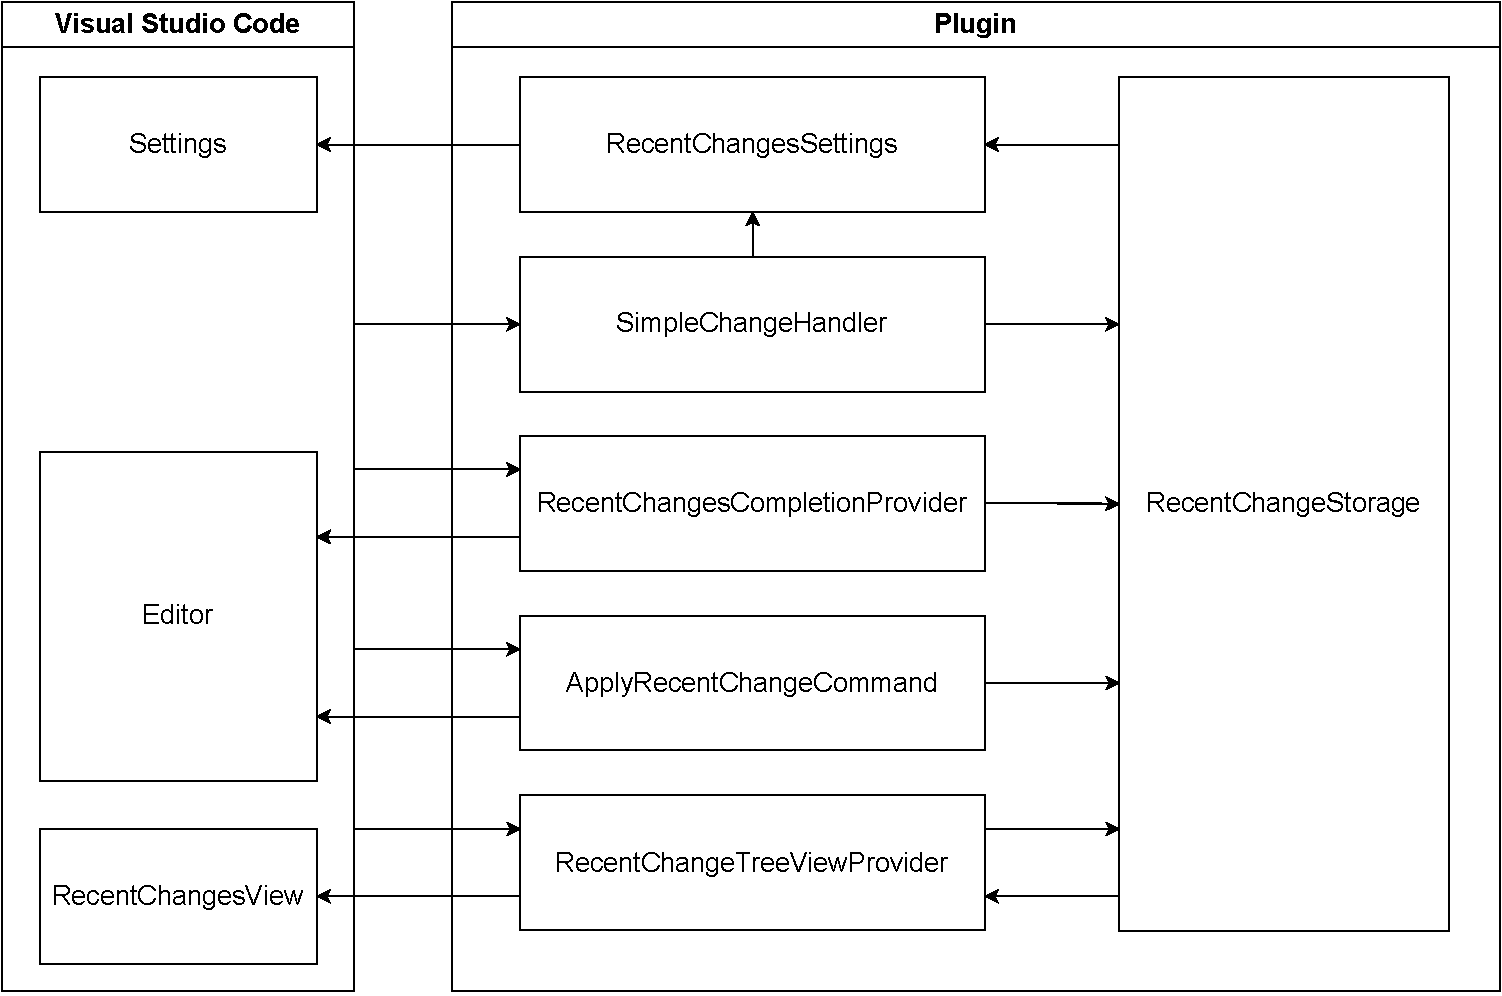
\includegraphics[width=.95\textwidth]{diagram_VSCodeDesign-Simplified}
    \caption{Stark vereinfachte Übersicht über das Design des Plugins in  VS Code.}
    \label{fig:diagram_VSCodeDesign-Simplified}
\end{figure}  

Das Herzstück des Plugins sind der \emph{SimpleChangeHandler} und
der \emph{RecentChangeStorage}. Der \emph{SimpleChangeHandler} hat die Aufgabe,
alle Veränderungen im geöffneten Dokument zu analysieren. Falls es sich um
eine verarbeitbare Veränderung handelt, wird diese im \emph{RecentChangeStorage}
gespeichert. Der \emph{RecentChangeStorage} bietet Methoden um die
gespeicherten Änderungen abzufragen und kümmert sich auch selber um das
Löschen von veralteten Änderungen.

Die Klasse \emph{RecentChangesSettings} bietet Zugriffsmethoden an,
um die von VS Code angebotenen Einstellungen abzufragen. Über sie
werden die Einstellungen für die \emph{QueueSize} (Anzahl von Veränderungen)
und die \emph{DebounceTime} (Debounce Zeit für das erkennen von Änderungen)
zugänglich gemacht.

Der \emph{RecentChangesCompletionProvider} implementiert die VS Code Schnittstelle
für Codevervollständigung. Er analysiert dabei das zu vervollständigende Wort
im Editor und fragt daraufhin den \emph{RecentChangesStorage} nach einer passenden
Änderung ab.

Der \emph{ApplyRecentChangeCommand} ist ein ausführbarer Command. Er ließt
das aktuelle Wort aus dem Editor aus, sucht im \emph{RecentChangesStorage}
nach einer passenden Änderung ersetzt und das Wort im Editor, falls
er fündig wird. Wird keine passende Änderung gefunden, so wird eine entsprechende
Nachricht angezeigt. Durch die Konfiguration des Plugins, kann der
Command auch über eine Tastenkombination aktiviert werden.

Der \emph{RecentChangesTreeViewProvider} implementiert eine Schnittstelle
um VS Code ein TreeView bereitzustellen. Die Daten für dieses TreeView
erhält er vom \emph{RecentChangesStorage}. Damit die TreeView aktuell
gehalten wird, wird der \emph{RecentChangesStorage} mithilfe eines Observer-Patterns % //TODO source
beobachtet und die TreeView bei Veränderungen aktualisiert.


% \begin{figure}
%     \centering
%     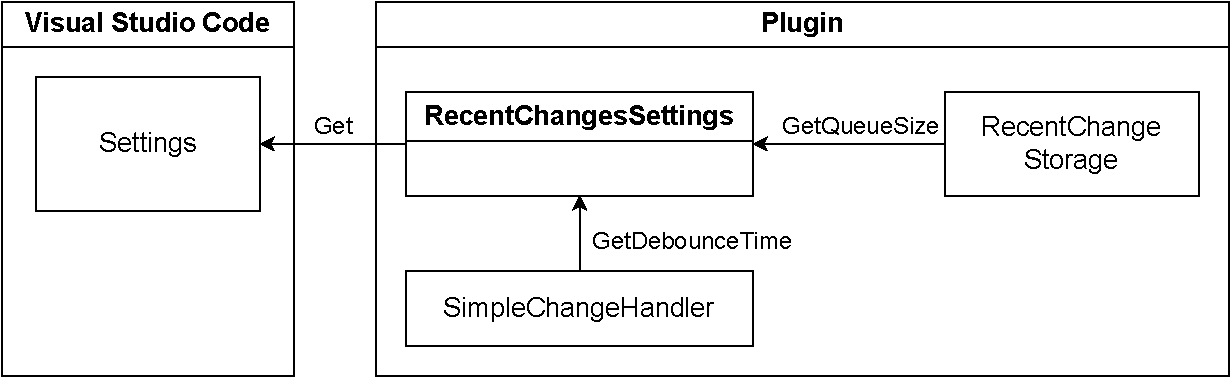
\includegraphics[width=.95\textwidth]{diagram_VSCodeDesign-Detail_Settings}
%     \caption{Detaillierte Darstellung der Komponente \emph{RecentChangesSettings}.}
%     \label{fig:diagram_VSCodeDesign-Detail_Settings}
% \end{figure} 
% \begin{figure}
%     \centering
%     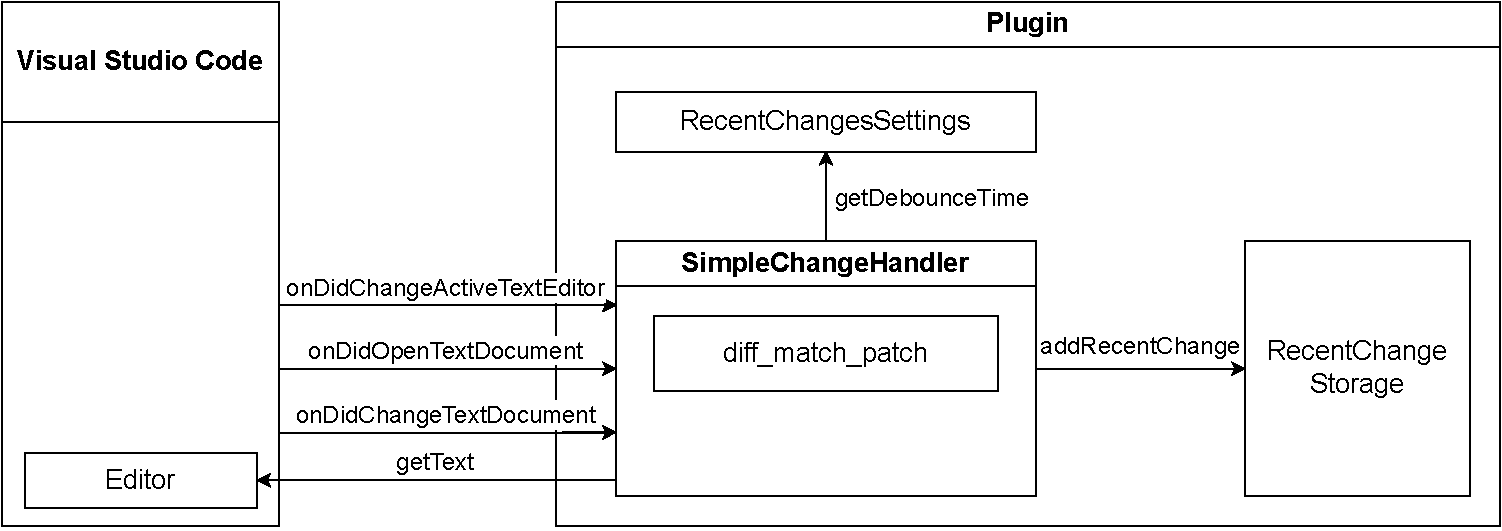
\includegraphics[width=.95\textwidth]{diagram_VSCodeDesign-Detail_Handler}
%     \caption{Detaillierte Darstellung des \emph{SimpleChangeHandler}.}
%     \label{fig:diagram_VSCodeDesign-Detail_Handler}
% \end{figure}
% \begin{figure}
%     \centering
%     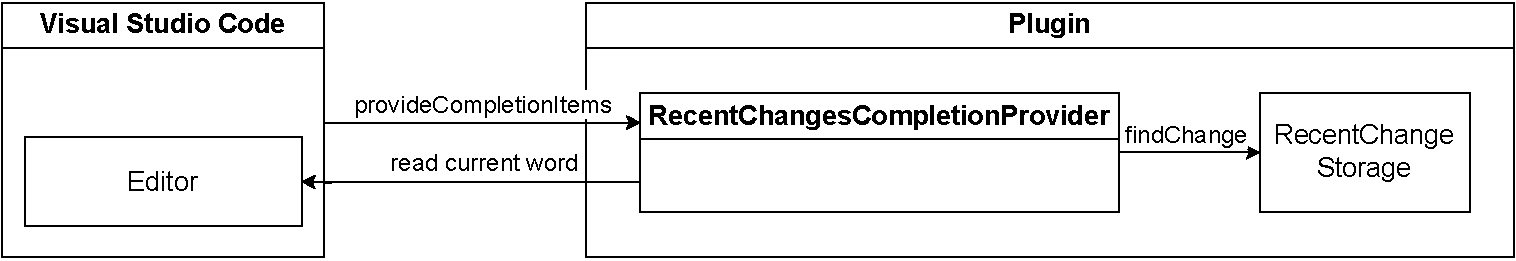
\includegraphics[width=.95\textwidth]{diagram_VSCodeDesign-Detail_Provider}
%     \caption{Detaillierte Darstellung des \emph{RecentChangesCompletionProvider}.}
%     \label{fig:diagram_VSCodeDesign-Detail_Provider}
% \end{figure}   
% \begin{figure}
%     \centering
%     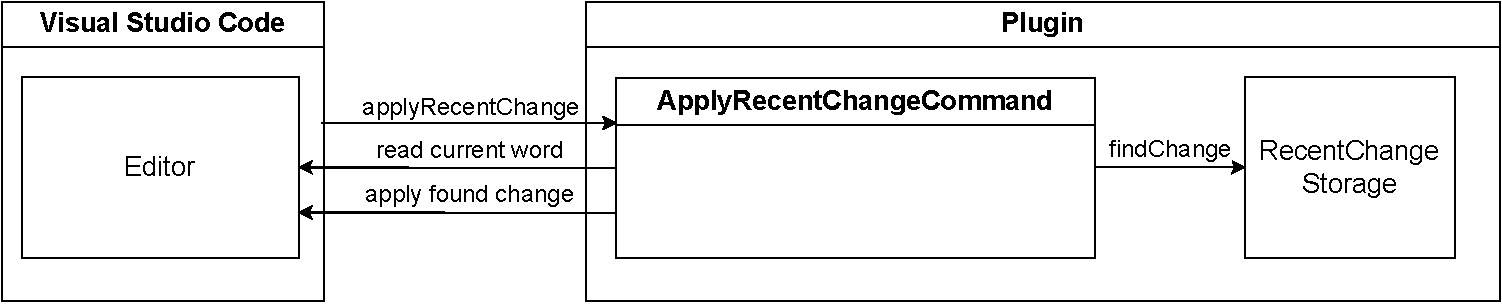
\includegraphics[width=.95\textwidth]{diagram_VSCodeDesign-Detail_Command}
%     \caption{Detaillierte Darstellung des \emph{ApplyRecentChangeCommand}.}
%     \label{fig:diagram_VSCodeDesign-Detail_Command}
% \end{figure}   
% \begin{figure}
%     \centering
%     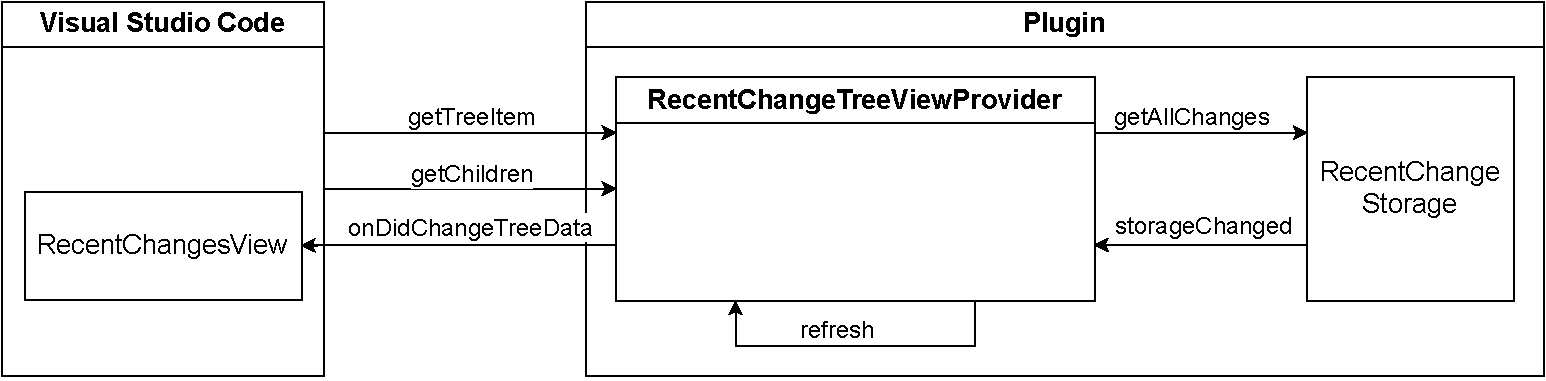
\includegraphics[width=.95\textwidth]{diagram_VSCodeDesign-Detail_TreeView}
%     \caption{Detaillierte Darstellung des \emph{RecentChangeTreeViewProvider}.}
%     \label{fig:diagram_VSCodeDesign-Detail_TreeView}
% \end{figure}   
% \begin{figure}
%     \centering
%     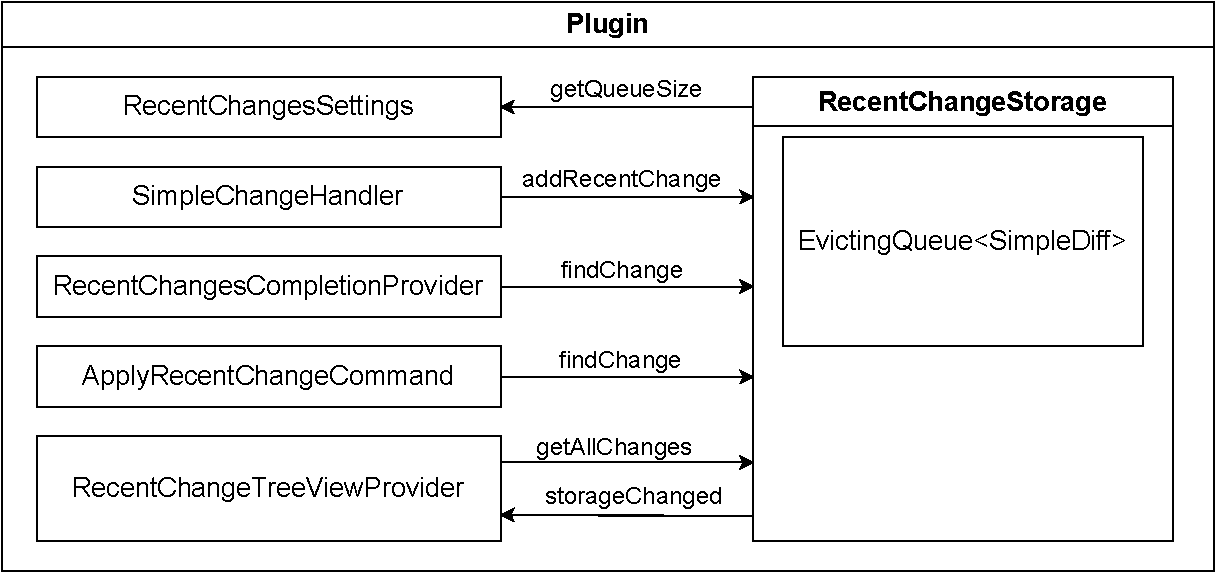
\includegraphics[width=.95\textwidth]{diagram_VSCodeDesign-Detail_Storage}
%     \caption{Detaillierte Darstellung des \emph{RecentChangeStorage}.}
%     \label{fig:diagram_VSCodeDesign-Detail_Storage}
% \end{figure}   

\section{Implementierung}
\label{sec:EntwicklungVsCode_Implementierung}

\subsection{Aufsetzen des Projektes}

\subsubsection{Aufbau der Ordnerstruktur}

\subsection{Entwicklung}

\section{Tests}
\label{sec:EntwicklungVsCode_Tests}

\section{Publishing}
\label{sec:EntwicklungVsCode_Publishing}

\section{CI/CD}
\label{sec:EntwicklungVsCode_CICD}